\documentclass[12pt]{letter}
\usepackage{amsmath,amsfonts,amsthm,amstext,amssymb,graphicx, multicol,fancyhdr,lastpage,fullpage,framed,fancybox,enumerate,tikz,color,mathrsfs, polynom}
\usepackage[margin=0.6in,headsep=3pt, headheight=15pt]{geometry}

% ----------------------------------------------------------
% Custom Definitions, Commands, Environments, etc.

% Sets of numbers
\def\R{\mathbb{R}} % The reals
\def\N{\mathbb{N}} % The naturals
\def\Z{\mathbb{Z}} % The integers
\def\Q{\mathbb{Q}} % The rationals

% Blank space
\newcommand{\blank}[1]{\underline{\hspace{#1}}} % Blank space

% Change font colors
\newcommand{\cyan}[1]{{\color{cyan}{#1}}} % Changes font to cyan
\newcommand{\red}[1]{{\color{red}{#1}}} % Changes font to red
\newcommand{\magenta}[1]{{\color{magenta}{#1}}} % Changes font to magenta
\newcommand{\orange}[1]{{\color{orange}{#1}}} % Changes font to orange
\newcommand{\yellow}[1]{{\color{yellow}{#1}}} % Changes font to yellow
\newcommand{\violet}[1]{{\color{violet}{#1}}} % Changes font to violet
\newcommand{\green}[1]{{\color{green}{#1}}} % Changes font to green
\newcommand{\blue}[1]{{\color{blue}{#1}}} % Changes font to blue
\newcommand{\white}[1]{{\color{white}{#1}}} % Changes font to white

% Fitted inclusion symbols
\newcommand{\fp}[1]{\left({#1}\right)} % Fitted parentheses around content
\newcommand{\fb}[1]{\left[{#1}\right]} % Fitted brackets
\newcommand{\set}[1]{\left\{{#1}\right\}} % Fitted braces (useful for sets)
\newcommand{\av}[1]{\left|{#1}\right|} % Fitted absolute value bars

% Augmented Matrix Environment
\newenvironment{amatrix}[1]{%
	\left[\begin{array}{@{}*{#1}{c}|c@{}}
	}{%
	\end{array}\right]
}

% Miscellaneous
\def\then{\Rightarrow}
\def\to{\rightarrow}
\def\d{^{\circ}}
\newcommand{\?}{\stackrel{?}{=}}



% Coordinate Plane (Four-Quadrant)
\def\coordplane {
	\begin{tikzpicture}		\draw[step=0.25cm,black,very thin,opacity=0.25] (-2.5cm, -2.5cm) grid (2.5cm, 2.5cm);
	\draw[<->,thick,black] (-2.5cm, 0) -- (2.5cm, 0) node[anchor=north west,pos=0.94,font=\scriptsize]{$x$};
	\draw[<->,thick,black] (0,-2.5cm) -- (0, 2.5cm) node[anchor=south east,font=\scriptsize,pos=0.94]{$y$};
	\end{tikzpicture}
}

% Coordinate Plane (One-Quadrant)
\def\onequad {
	\begin{tikzpicture}
	\draw[step=0.25cm, black, very thin, opacity=0.25] (0,0) grid (7.5cm,5cm);
	\draw[->, thick, black] (0,0) -- (7.5cm, 0) node[anchor=north west,font=\scriptsize,pos=0.94]{$x$};
	\draw[->, black, thick] (0,0) -- (0,5cm) node[anchor=south east,font=\scriptsize,pos=0.94]{$y$};
	\end{tikzpicture}
}

% Counters
\newcounter{exercise}

% Exercise environment (auto-numbered)
\newenvironment{exercise}[1][]{\begin{framed}\refstepcounter{exercise}\textbf{Exercise~\theexercise:} #1}{\end{framed}}

% Book exercise environment
\newenvironment{bex}[2][] {
	\begin{framed}
		\textbf{Book Exercise {#2}}#1
	\end{framed}
}
% ----------------------------------------------------------

% ----------------------------------------------------------
% Header and Footer Information
% \pagestyle{fancy}
% \fancyhf{}
% \renewcommand{\headrulewidth}{0pt}
% \rhead{Name: \blank{2in}}
% \lhead{@}
% \rfoot{Page \thepage \, of \,\pageref{LastPage}}
% ----------------------------------------------------------
\author{Jacob Ayers}

\begin{document}
	\textbf{Assignment 8 Key \\ MAT 130}
	
	\begin{bex}{4.2.16}
		{
			
		}
	\end{bex} \vspace{-8pt}
	
	% My answer here
	(a) Domain: $x \neq 3$
	
	(b) Since the numerator will never be zero, there are no $x$-intercepts. To find the $y$-intercept, set $x = 0$ and solve for $y$. $y = \dfrac{1}{0 - 3} = -\dfrac13$, so there is a $y$-intercept at $\fp{0, -\dfrac13}$.
	
	(c) There is a vertical asymptote at $x = 3$ and since the degree of the denominator is larger than the degree of the numerator, there is a horizontal asymptote at $y = 0$.
	
	(d) We only have one point currently, so we need several additional points (a few on each side of the vertical asymptote). I used a graphing calculator to find the following:
	
	\begin{tabular}{c|cccccccc}
		$x$ & $-1$ & $1$ & $2$ & $2.5$ & $3.5$ & $4$ & $5$ & $6$ \\ \hline
		$f(x)$ & $-0.25$ & $-0.5$ & $-1$ & $-2$ & $2$ & $1$ & $0.5$ & $0.33$
	\end{tabular}

	Using this information, we can get a very accurate sketch: \\
	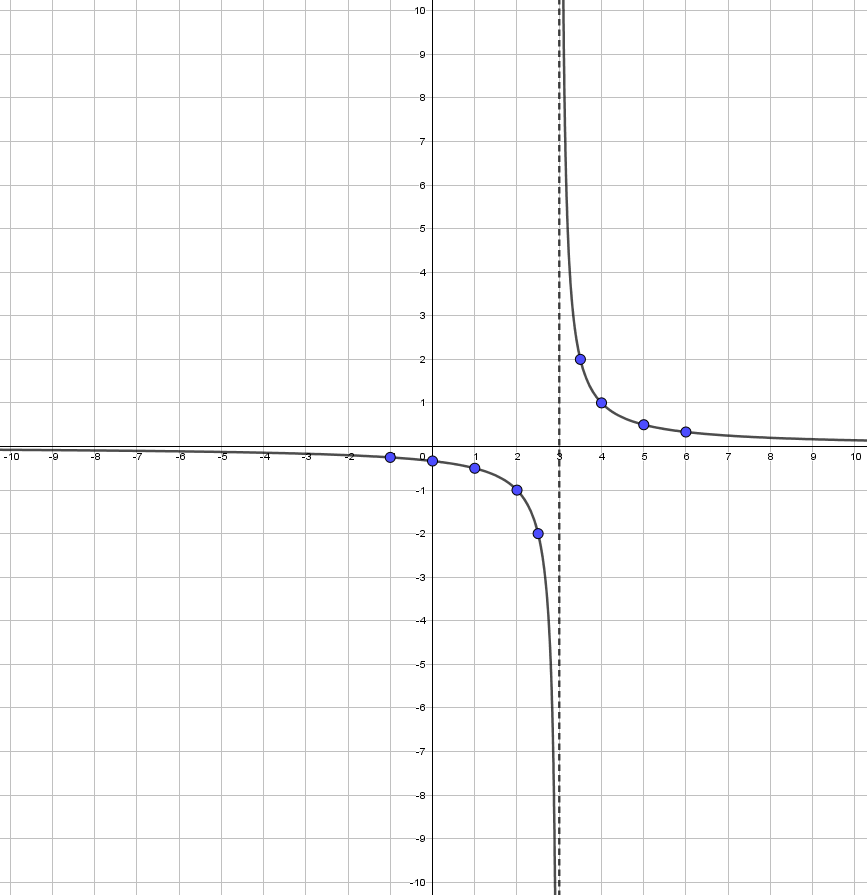
\includegraphics[width=3in]{4216.png}
	
	\vfill \newpage
	
	\begin{bex}{4.2.20}
		{
			
		}
	\end{bex} \vspace{-8pt}
	
	% My answer here
	First, rewrite the numerator and denominator in standard form: $f(x) = \dfrac{-3x + 1}{-x + 1}$
	
	(a) Domain: $x \neq 1$
	
	(b) The numerator is zero when $x = \dfrac13$, so the $x$-intercept of the graph is $\fp{\dfrac13, 0}$. If we set $x = 0$, then $P(0) = \dfrac{-3(0) + 1}{-(0) + 1} = 1$, so the $y$-intercept of the graph is $(0, 1)$
	
	(c) There is a vertical asymptote at $x = 1$ and since the degrees of the numerator and denominator are equal, there is a horizontal asymptote at $y = \dfrac{-3}{-1} = 3$.
	
	(d) We have a couple points to the left of the vertical asymptote, but we could use a couple more. We have no points on the right side of the vertical asymptote, so we'll need several of those.
	
	\begin{tabular}{c|cccccc}
		$x$ & $-1$ & $-2$ & $1.5$ & $2$ & $3$ & $4$ \\ \hline
		$f(x)$ & $2$ & $2.33$ & $7$ & $5$ & $4$ & $3.67$
	\end{tabular}

	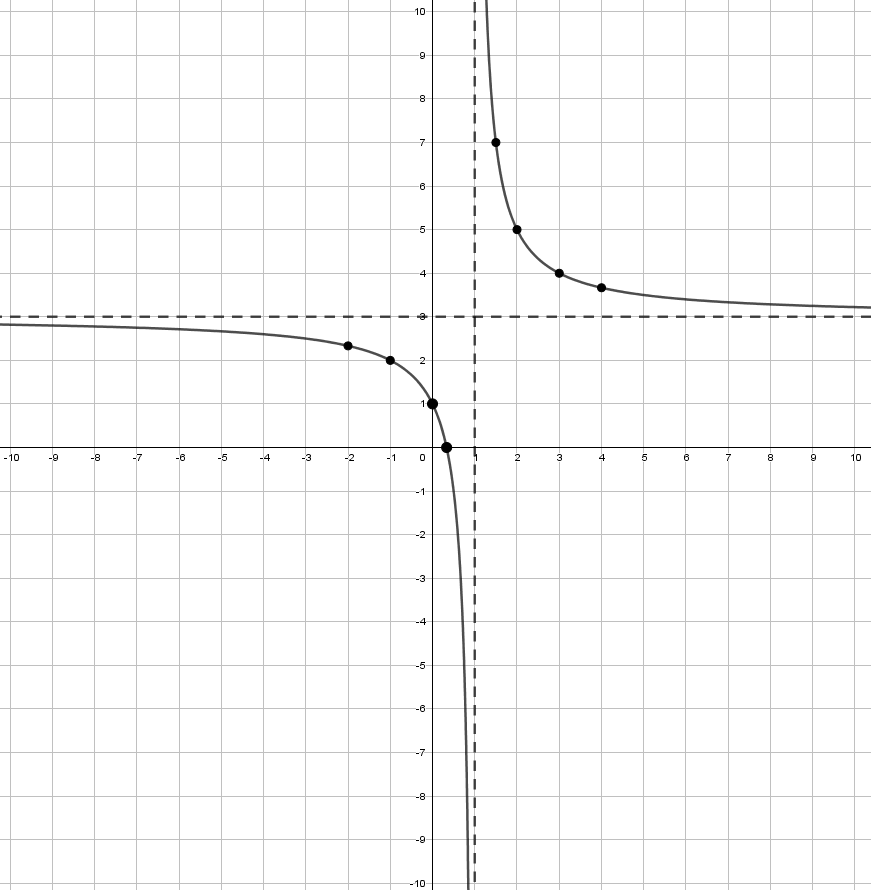
\includegraphics[width=3in]{4220.png}
	
	\vfill \newpage
	
	\begin{bex}{4.2.24}
		{
			
		}
	\end{bex} \vspace{-8pt}
	
	% My answer here
	First, rewrite the numerator in standard form: $f(t) = \dfrac{-2t + 1}{t}$.
	
	(a) Domain: $x \neq 0$
	
	(b) $x$-intercept: $\fp{\dfrac12, 0}$ \\
		No $y$-intercept since $f(0)$ is undefined.
		
	(c) Vertical asymptote at $x = 0$ \\
		Horizontal asymptote at $y = \dfrac{-2}{1} = -2$
		
	(d) \begin{tabular}{c|ccccccc}
		$t$ & $-3$ & $-2$ & $-1$ & $-0.5$ & $1$ & $2$ & $3$ \\ \hline
		$f(t)$ & $-2.33$ & $-2.5$ & $-3$ & $-4$ & $-1$ & $-1.5$ & $-1.67$
	\end{tabular}

	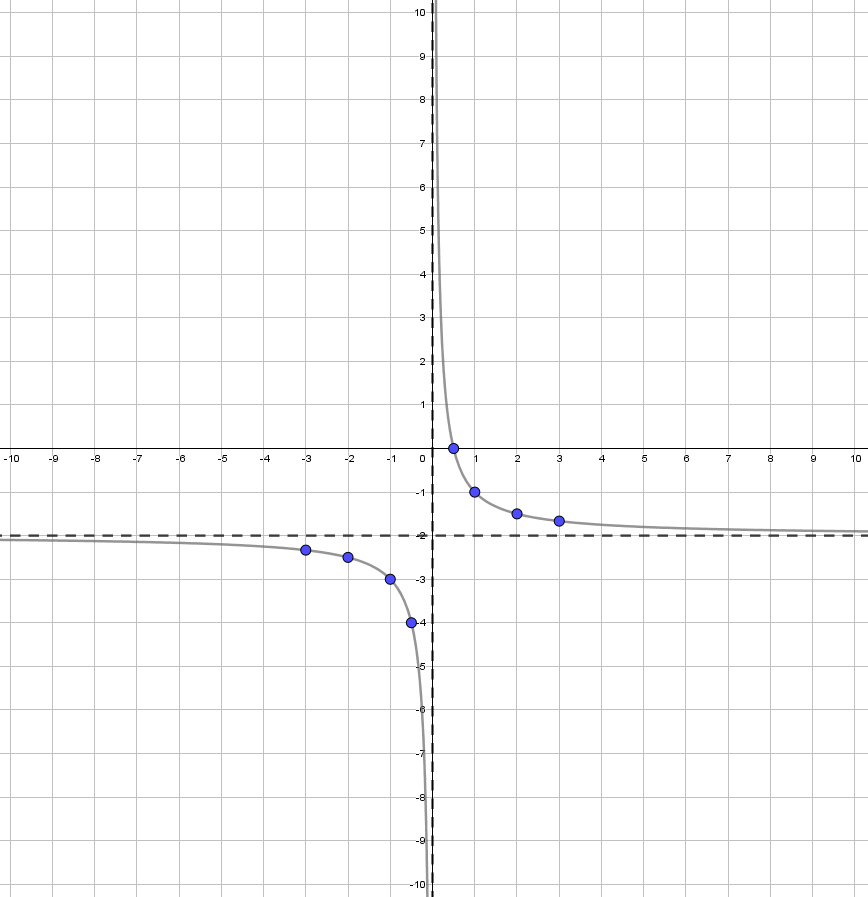
\includegraphics[width=3in]{4224.png}
	
	\vfill \newpage
	
	\begin{bex}{4.2.28}
		{
			
		}
	\end{bex} \vspace{-8pt}
	
	% My answer here
	(a) Domain: $x \neq 2$
	
	(b) $x$-intercept: $(0, 0)$ \\
		$y$-intercept: $(0,0)$ 
		
	(c) Vertical asymptote at $x = 2$ \\
		Horizontal asymptote at $y = 0$
		
	(d) \begin{tabular}{c|cccccccc}
		$x$ & $-2$ & $-1$ & $1$ & $1.5$ & $2.5$ & $3$ & $4$ & $5$ \\ \hline
		$f(x)$ & $0.13$ & $0.11$ & $-1$ & $-6$ & $-10$ & $-3$ & $-1$ & $-0.56$
	\end{tabular}

	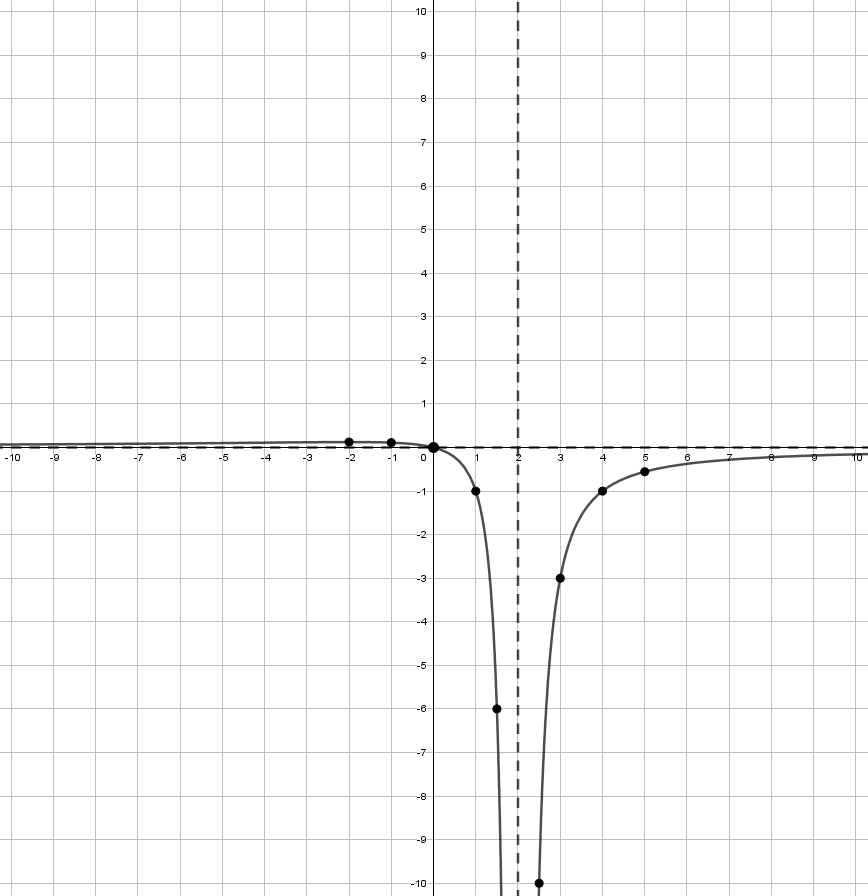
\includegraphics[width=3in]{4228.png}
	
	\vfill \newpage
	
	\begin{bex}{4.2.32}
		{
			
		}
	\end{bex} \vspace{-8pt}
	
	% My answer here
	(a) Domain: $x \neq -3, 1$
	
	(b) $x$-intercept: $(0,0)$ \\
		$y$-intercept: $(0,0)$
		
	(c) Vertical asymptotes at $x = -3$ and $x = 1$ \\
		Horizontal asymptote at $y = 0$
		
	(d) \begin{tabular}{c|cccccccccccc}
		$x$ & $-6$ & $-5$ & $-4$ & $-3.5$ & $-2.5$ & $-2$ & $-1$ & $0.5$ & $1.5$ & $2$ & $3$ & $4$ \\ \hline
		$f(x)$ & $-0.86$ & $-1.25$ & $-2.4$ & $-4.67$ & $4.29$ & $2$ & $0.75$ & $-0.86$ & $2$ & $1.2$ & $0.75$ & $0.57$
	\end{tabular}

	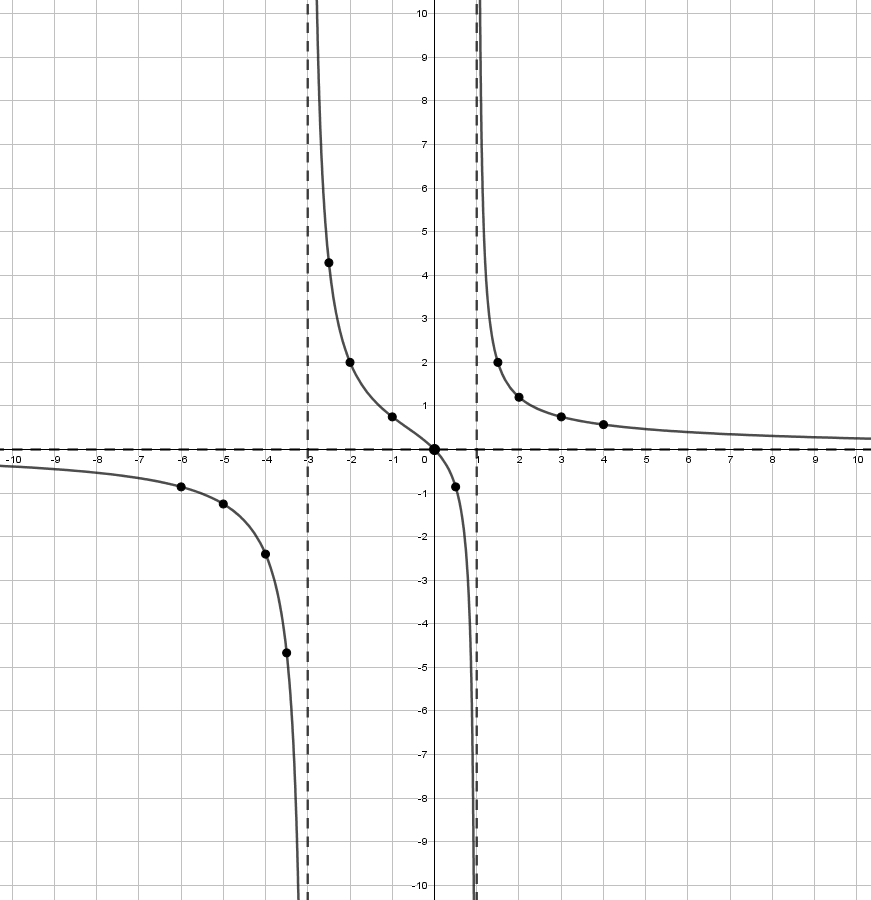
\includegraphics[width=3in]{4232.png}
	
	\vfill \newpage
	
	\begin{bex}{4.2.36}
		{
			
		}
	\end{bex} \vspace{-8pt}
	
	% My answer here
	First, simplify: $\dfrac{x^2 - 36}{x + 6} = \dfrac{(x+6)(x-6)}{x + 6} = x - 6$
	
	(a) Domain: $x \neq -6$ (will be a hole)
	
	(b) $x$-intercept: $(6, 0)$ \\
		$y$-intercept: $(0, -6)$
		
	(c) Lines don't have asymptotes
	
	(d) We only need two points in order to graph a line; no further points needed
	
	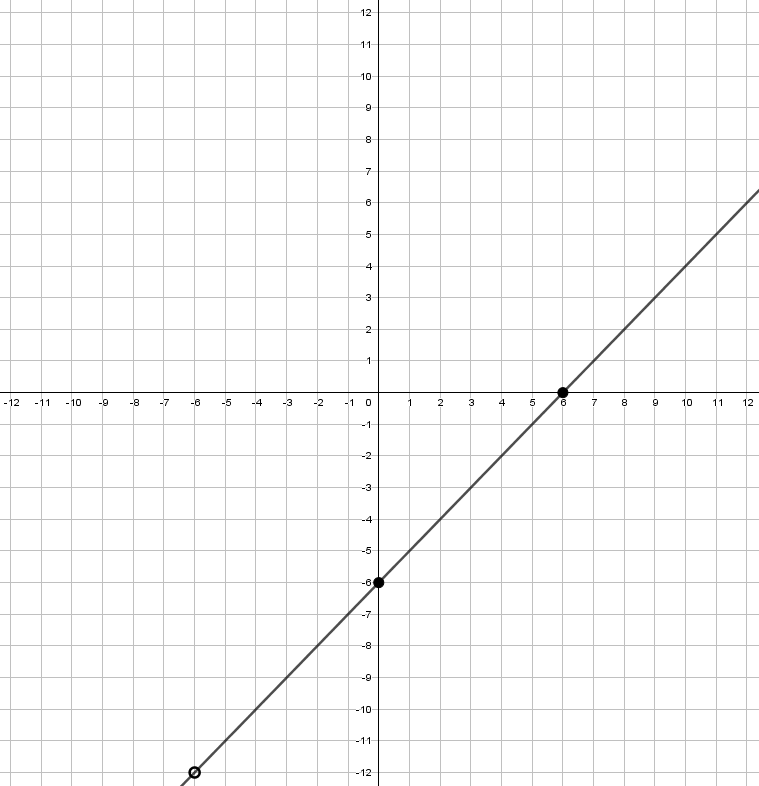
\includegraphics[width=3in]{4236.png}
	
	\vfill \newpage
	
	\begin{bex}{4.2.40}
		{
			
		}
	\end{bex} \vspace{-8pt}
	
	% My answer here
	(a) Domain: $x \neq -5, 3$
	
	(b) No $x$-intercept since the numerator will never be zero \\
		$y$-intercept: $\fp{0, -\dfrac15}$
		
	(c) Vertical asymptotes at $x = -5$ and $x = 3$ \\
		Horizontal asymptote at $y = \dfrac{3}{1} = 3$
		
	(d) \begin{tabular}{c|cccccccccccccccc}
		$x$ & -8 & -7 & -6 & -5.5 & -4.5 & -4 & -3 & -2 & -1 & 1 & 2 & 2.5 & 3.5 & 4 & 5 & 6 \\ \hline
		$f(x)$ & 5.91 & 7.5 & 12.33 & 22.06 & -17 & -7.29 & -2.5 & -1 & -0.38 & -0.5 & -2.14 & -5.8 & 9.35 & 5.67 & 3.9 & 3.36
	\end{tabular}

	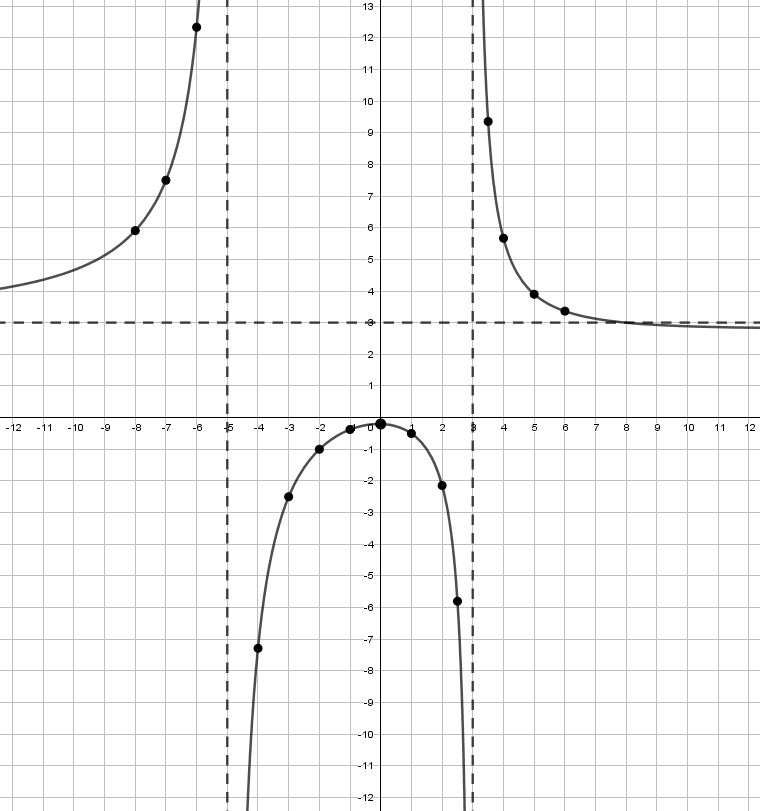
\includegraphics[width=3in]{4240.png}
	
	\vfill \newpage
	
	\begin{bex}{4.2.44}
		{
			
		}
	\end{bex} \vspace{-8pt}
	
	% My answer here
	In order to find the domain and any vertical asymptotes, we'll need to find the zeros of the denominator. Unfortunately, it's not factorable and it's a cubic so we'll need to use the Rational Zero Test and synthetic division to find one zero and then factor or use the quadratic formula on what's left to find the other two zeros.
	
	Possible rational zeros: $\pm 1, \pm 2, \pm 3, \pm 6$ (factors of 6; denominator must always be 1)
	
	$\polyhornerscheme[x=1]{x^3 - 2x^2 - 5x + 6}$
	
	So $x^3 - 2x^2 - 5x + 6 = (x - 1)(x^2 - x - 6) = (x - 1)(x-3)(x+2)$.
	
	Simplifying: $\dfrac{x^2 - x - 2}{x^3 - 2x^2 - 5x + 6} = \dfrac{(x - 2)(x+1)}{(x-1)(x-3)(x+2)}$
	
	(a) Domain: $x \neq -2, 1, 3$
	
	(b) $x$-intercepts: $(-1, 0)$ and $(2, 0)$ \\
		$y$-intercept: $\fp{0, -\dfrac13}$
		
	(c) Vertical asymptotes at $x = -2$, $x = 1$, and $x = 3$ \\
		Horizontal asymptote at $y = 0$
		
	(d) \begin{tabular}{c|cccccccccccc}
		$x$ & -5 & -4 & -3 & -2.5 & -1.5 & 0.5 & 1.5 & 2.5 & 3.5 & 4 & 5 & 6 \\ \hline
		$f(x)$ & -0.19 & -0.26 & -0.42 & -0.7 & 0.31 & -0.72 & 0.48 & -0.52 & 0.98 & 0.56 & 0.32 & 0.23
	\end{tabular}

	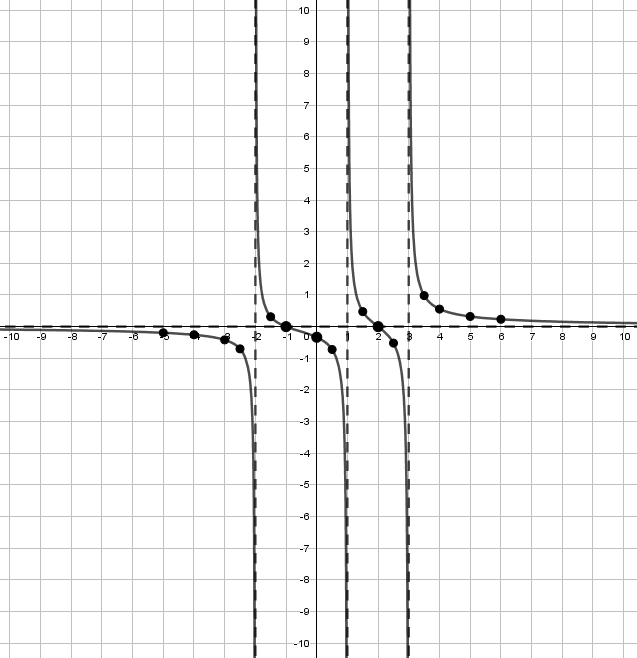
\includegraphics[width=3in]{4244.png}
	
	\vfill \newpage
	
	\begin{bex}{4.2.48}
		{
			
		}
	\end{bex} \vspace{-8pt}
	
	% My answer here
	$\polylongdiv{x^2 + 5}{x}$
	
	So $\dfrac{x^2 + 5}{x} = x + \dfrac{5}{x}$.
	
	(a) Domain: $x \neq 0$
	
	(b) No $x$-intercept since numerator will never be zero \\
		No $y$-intercept since $g(0)$ is undefined
		
	(c) Vertical asymptote at $x = 0$ \\
		Slant asymptote at $y = x$
		
	(d) \begin{tabular}{c|cccccccccccc}
		$x$ & -6 & -5 & -4 & -3 & -2 & -1 & 1 & 2 & 3 & 4 & 5 & 6 \\ \hline
		$f(x)$ & -6.83 & -6 & -5.25 & -4.67 & -4.5 & -6 & 6 & 4.5 & 4.67 & 5.25 & 6 & 6.83
	\end{tabular}
	
	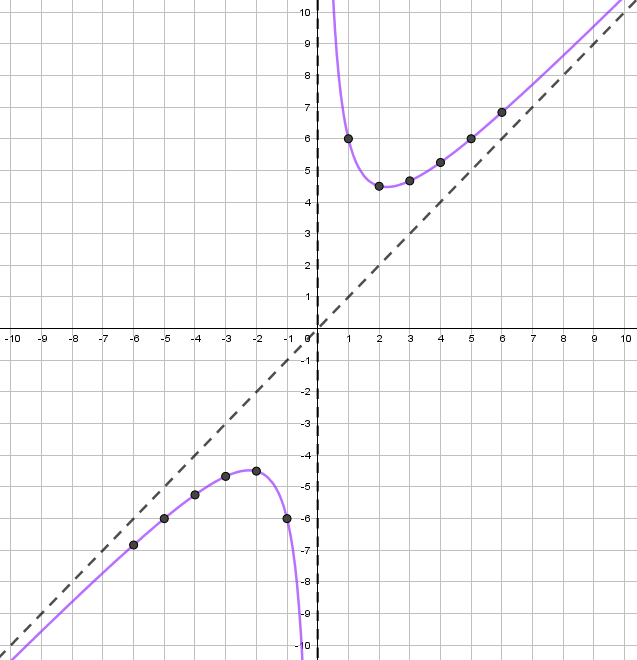
\includegraphics[width=3in]{4248.png}
	
	\vfill \newpage
	
	\begin{bex}{4.2.56}
		{
			
		}
	\end{bex} \vspace{-8pt}
	
	% My answer here
	$\polylongdiv{x^3}{2x^2 - 8}$
	
	So $\dfrac{x^3}{2x^2 - 8} = \dfrac12 x + \dfrac{4x}{2x^2 - 8}$.
	
	Simplifying: $\dfrac{x^3}{2x^2 - 8} = \dfrac{x^3}{2(x^2 - 4)} = \dfrac{x^3}{2(x+2)(x-2)}$
	
	(a) Domain: $x \neq \pm 2$
	
	(b) $x$-intercept and $y$-intercept: $(0, 0)$
	
	(c) Vertical asymptotes at $x = -2$ and $x = 2$ \\
		Slant asymptote at $y = \dfrac12 x$
		
	(d) \begin{tabular}{c|cccccccccccc}
		$x$ & -5 & -4 & -3 & -2.5 & -1.5 & -1 & 1 & 1.5 & 2.5 & 3 & 4 & 5 \\ \hline
		$g(x)$ & -2.98 & -2.67 & -2.7 & -3.47 & 0.96 & 0.17 & -0.17 & -0.96 & 3.47 & 2.7 & 2.67 & 2.98
	\end{tabular}

	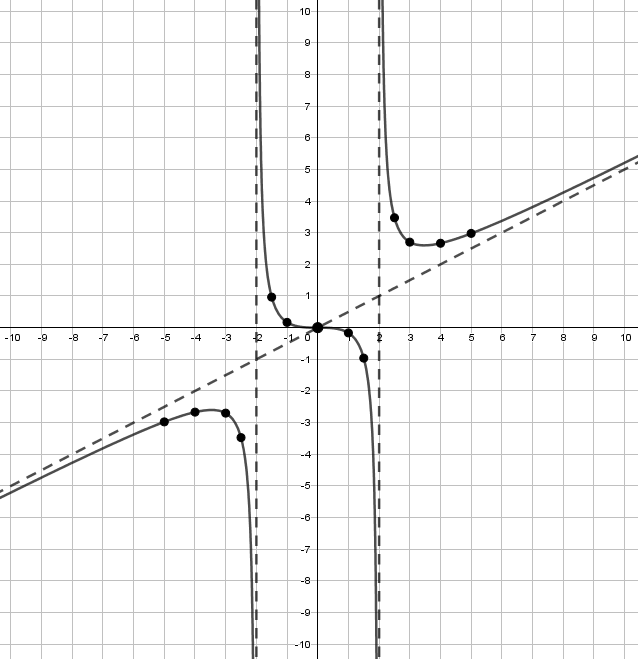
\includegraphics[width=3in]{4256.png}
	
	\vfill \newpage
	
	\begin{bex}{4.2.88}
		{
			
		}
	\end{bex} \vspace{-8pt}
	
	% My answer here
	Domain: $x > 0$
	
	The average cost will always be positive (i.e. $\overline{C} > 0$) so we can use a one-quadrant graph to graph this function. To graph it, we will use the point-plotting method.
	
	\begin{tabular}{c|cccccccc}
		$x$ & 1 & 2 & 3 & 4 & 5 & 6 & 7 & 8 \\ \hline
		$\overline{C}$ & 15.2 & 12.9 & 12.27 & 12.05 & 12 & 12.03 & 12.11 & 12.23
	\end{tabular}

	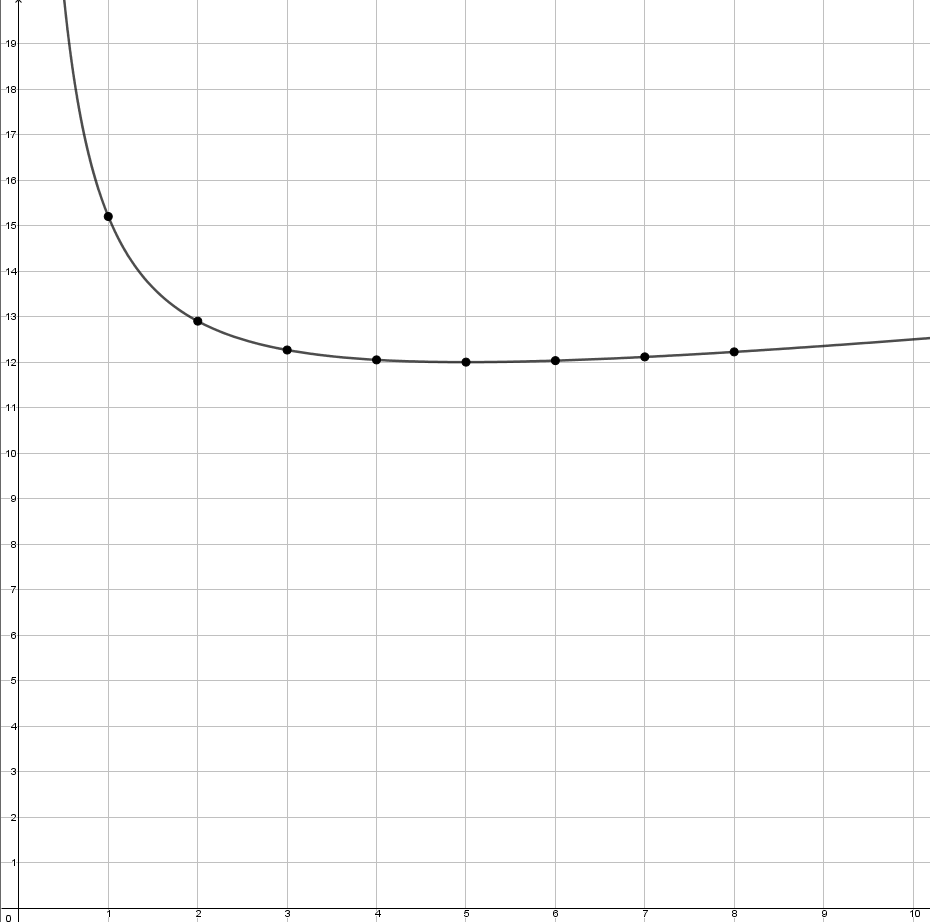
\includegraphics[width=3in]{4288.png}
	
	In order to minimize the average cost per unit, 5 units should be produced.
	
	\vfill % \newpage
	
	\begin{bex}{5.1.12}
		{
			
		}
	\end{bex} \vspace{-32pt}
	
	% My answer here
	\begin{flalign*}
	200(1.02)^{12(24)} &= 200(1.2)^{288} & \\
	&= 200\fp{299.8123147} & \\
	&\approx 59962.463
	\end{flalign*}
	
	\vfill \newpage
	
	\begin{bex}{5.1.18}
		{
			
		}
	\end{bex} \vspace{-8pt}
	
	% My answer here
	\begin{tabular}{c|ccccccc}
		$x$ & 3 & 2 & 1 & 0 & -1 & -2 & -3 \\ \hline
		$f(x)$ & $\dfrac{1}{343}$ & $\dfrac{1}{49}$ & $\dfrac17$ & 1 & 7 & 49 & 343
	\end{tabular}

	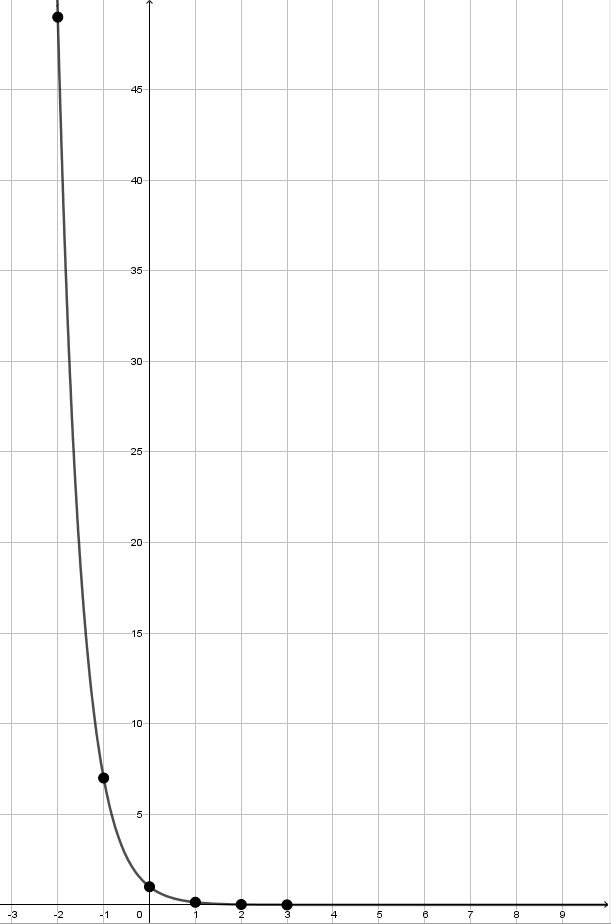
\includegraphics[width=2in]{5118.png}
	
	\vfill % \newpage
	
	\begin{bex}{5.1.22}
		{
			
		}
	\end{bex} \vspace{-8pt}
	
	% My answer here
	\begin{tabular}{c|ccccccc}
		$x$ & 2 & 1 & 0 & -1 & -2 & -3 & -4 \\ \hline
		$f(x)$ & 64 & 16 & 4 & 1 & $\dfrac14$ & $\dfrac{1}{16}$ & $\dfrac{1}{64}$
	\end{tabular}

	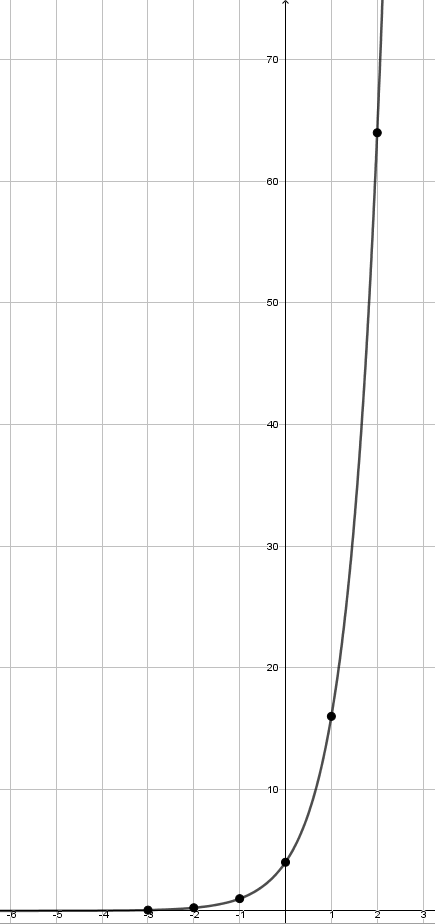
\includegraphics[width=1.5in]{5122.png}
	
	\vfill \newpage
	
	\begin{bex}{5.1.26}
		{
			
		}
	\end{bex} \vspace{-32pt}
	
	% My answer here
	\begin{flalign*}
	2^{x-2} &= 64 & \\
	2^{x-2} &= 2^6 & \\
	x - 2 &= 6 & \\
	x &= 8
	\end{flalign*}
	
	\vfill % \newpage
	
	\begin{bex}{5.1.28}
		{
			
		}
	\end{bex} \vspace{-32pt}
	
	% My answer here
	\begin{flalign*}
	5^{x-2} &= \dfrac{1}{125} & \\
	5^{x-2} &= 5^{-3} & \\
	x - 2 &= -3 & \\
	x &= -1
	\end{flalign*}
	
	\vfill % \newpage
	
	\begin{bex}{5.1.35}
		{
			
		}
	\end{bex} \vspace{-32pt}
	
	% My answer here
	\begin{flalign*}
	5000e^{0.06(6)} &= 5000e^{0.36} & \\
	&\approx 7166.647
	\end{flalign*}
	
	\vfill % \newpage
	
	\begin{bex}{5.1.46}
		{
			
		}
	\end{bex} \vspace{-8pt}
	
	% My answer here
	$2x - 1 = 4 \then x = \dfrac52$
	
	\vfill \newpage
	
	\begin{bex}{5.1.52}
		{
			
		}
	\end{bex} \vspace{-32pt}
	
	% My answer here
	\begin{flalign*}
	A &= 1000\fp{1 + \dfrac{0.06}{1}}^{40(1)} & \\
	&= 1000(1.06)^{40} & \\
	&\approx 10285.72
	\end{flalign*} \vspace{-24pt}
	\begin{flalign*}
	A &= 1000\fp{a + \dfrac{0.06}{2}}^{40(2)} & \\
	&= 1000(1.03)^{80} & \\
	&\approx 10640.89
	\end{flalign*} \vspace{-24pt}
	\begin{flalign*}
	A &= 1000\fp{1 + \dfrac{0.06}{4}}^{40(4)} & \\
	&= 1000(1.015)^{160} & \\
	&\approx 10828.46
	\end{flalign*} \vspace{-24pt}
	\begin{flalign*}
	A &= 1000\fp{1 + \dfrac{0.06}{12}}^{40(12)} & \\
	&= 1000\fp{1.005}^{480} & \\
	&\approx 10957.45
	\end{flalign*} \vspace{-24pt}
	\begin{flalign*}
	A &= 1000\fp{1 + \dfrac{0.06}{365}}^{40(365)} & \\
	&= 1000(1.00016438)^{14600} & \\
	&\approx 11021.00
	\end{flalign*} \vspace{-24pt}
	\begin{flalign*}
	A &= 1000e^{0.06(40)} & \\
	&= 1000e^{2.4} & \\
	&\approx 11023.18
	\end{flalign*}
	
	\vfill % \newpage
	
	\begin{bex}{5.1.58}
		{
			
		}
	\end{bex} \vspace{-8pt}
	
	% My answer here
	$P = 5000$, $r = 0.075$, $t = 50$
	\begin{flalign*}
	A &= 5000e^{0.075(50)} & \\
	&= 5000e^{3.75} & \\
	&\approx 212605.41
	\end{flalign*}
	
	\vfill \newpage
	
	\begin{bex}{5.1.60}
		{
			
		}
	\end{bex} \vspace{-8pt}
	
	% My answer here
	(a) $V(1) = 100e^{4.6052} \approx 10000$
	
	(b) $V(1.5) = 100e^{4.6052(1.5)} = 100e^{6.9078} \approx 100004$
	
	(c) $V(2) = 100e^{4.6052(2)} = 100e^{9.2104} \approx 1000060$
	
	\vfill % \newpage
	
	\begin{bex}{5.1.62}
		{
			
		}
	\end{bex} \vspace{-8pt}
	
	% My answer here
	(a) Looking at the formula, we are multiplying a constant (57.59) by a variable term that will increase in value as $t$ increases. So the population of Italy is increasing over time.
	
	(b and c) We need to evaluate $P(3)$, $P(15)$, $P(20)$, and $P(25)$. I used a graphing calculator to find the values.
	
	\begin{tabular}{c|cccc}
		Year & 2003 & 2015 & 2020 & 2025 \\ \hline
		Population (millions) & $58.478$ & $62.169$ & $63.774$ & $65.421$
	\end{tabular}
	
	\vfill \newpage
	
	\begin{bex}{5.1.64}
		{
			
		}
	\end{bex} \vspace{-8pt}
	
	% My answer here
	(a and b) We need to evaluate $Q(0)$ and $Q(2000)$. I used a graphing calculator to find the values (along with other values that we'll use to sketch the graph in part c).
	
	\begin{tabular}{c|ccccccccccc}
		Time (years) & 0 & 1000 & 2000 & 3000 & 4000 & 5000 & 6000 & 7000 & 8000 & 9000 & 10000 \\ \hline
		Amount Present & 10 & 8.8578 & 7.8461 & 6.9499 & 6.1561 & 5.4530 & 4.8301 & 4.2784 & 3.898 & 3.3569 & 2.9735
	\end{tabular}

	(c)
	
	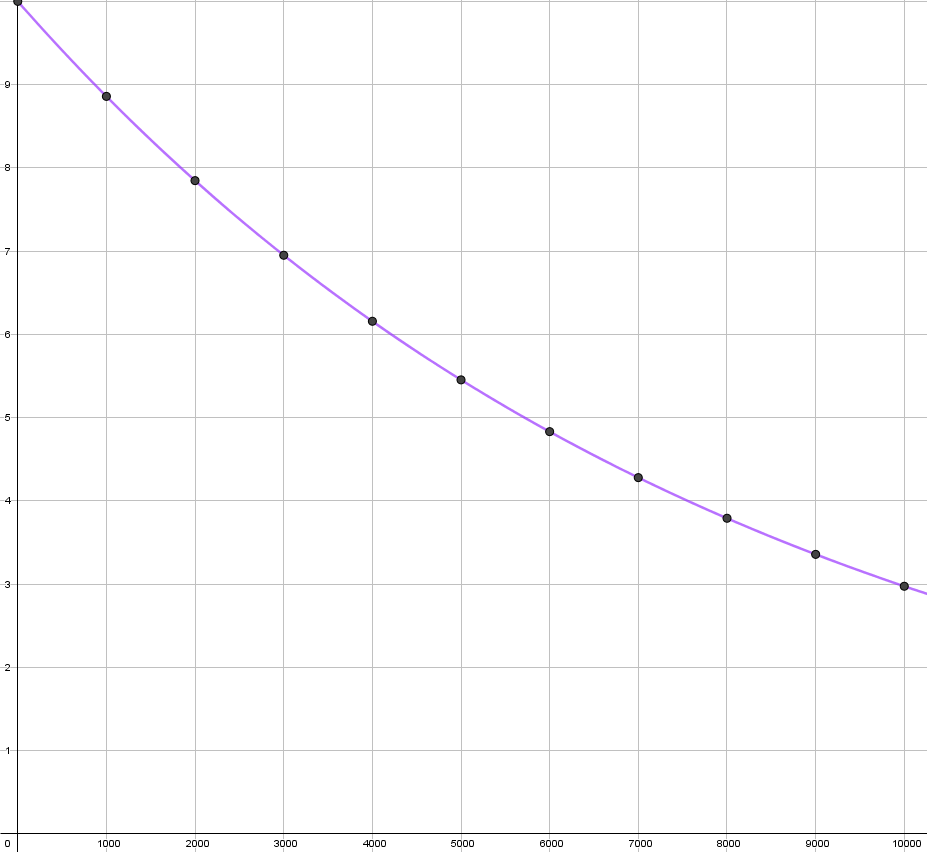
\includegraphics[width=3in]{5164c.png}
	
	\vfill % \newpage
	
	
	
\end{document}